\begin{figure}[h]
\centering
    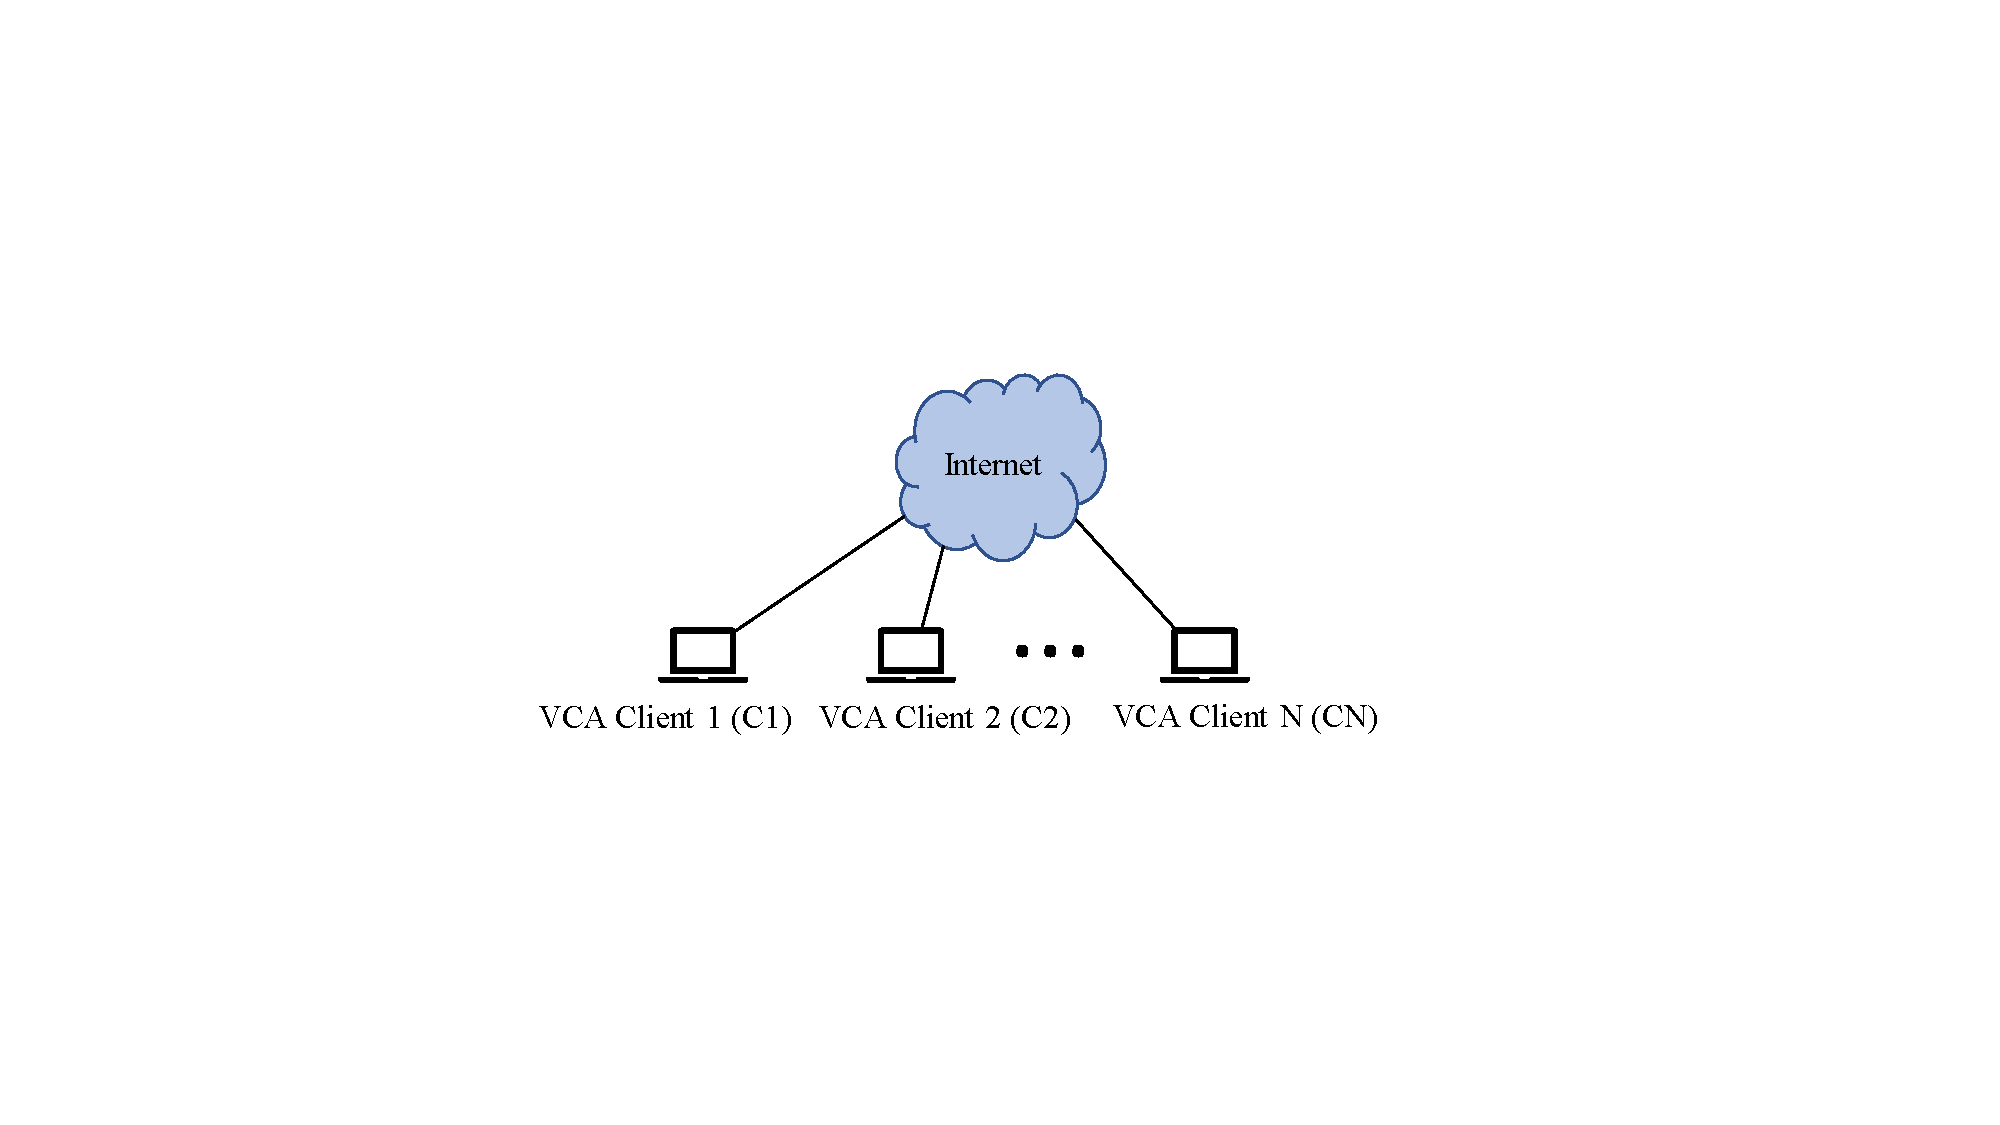
\includegraphics[width=0.35\textwidth,keepaspectratio]{../figures/methodology/modality-setup.pdf}
    \caption{Setup for modality experiments. All clients are connected a single call via a cloud server.}
    \label{fig:modality-setup}
\end{figure}

\begin{figure*}[ht]
\begin{subfigure}[t]{.33\textwidth}
  \centering
   \captionsetup{width=.9\linewidth}
    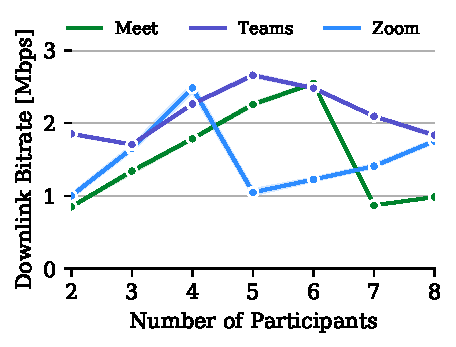
\includegraphics[width=1\textwidth,keepaspectratio]{../figures/modality/speaker_recv.pdf}
    \caption{Downlink traffic of client whose video is viewed in gallery mode}
    \label{fig:gallery-recv}
\end{subfigure}
\hfill
\begin{subfigure}[t]{.33\textwidth}
  \centering
   \captionsetup{width=.9\linewidth}
    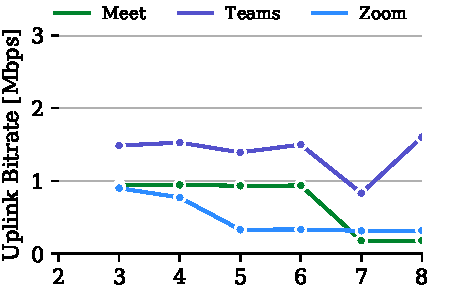
\includegraphics[width=1\textwidth,keepaspectratio]{../figures/modality/gallery_send.pdf}
    \caption{Uplink traffic of client whose video is viewed in gallery mode}
    \label{fig:gallery-send}
\end{subfigure}
\hfill
\begin{subfigure}[t]{.33\textwidth}
  \centering
   \captionsetup{width=.9\linewidth}
    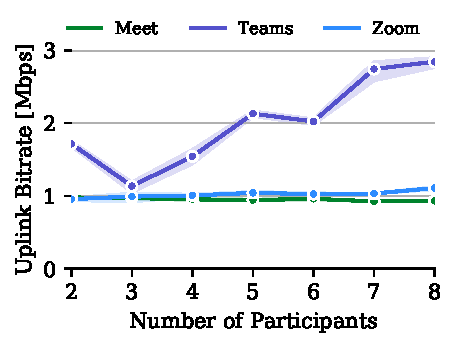
\includegraphics[width=1\textwidth,keepaspectratio]{../figures/modality/speaker_send.pdf}
    \caption{Uplink traffic of client whose video is pinned by all other participants}
    \label{fig:speaker-send}
\end{subfigure}
\caption{Network utilization in different viewing modalities}
\label{fig:viewing-mode}
\end{figure*}

\section{Call parameters and 
consumption}\label{sec:usage_modality}





%Until now, we have focused on the performance and network utilization of 2-person calls.

The way in which VCAs are used has changed over time, especially in the last year due to the COVID-19. For instance, it is more common to have large number of participants, especially in a work or school context. We now look at network utilization under two prominent call modalities: the number of participants in a call and the viewing mode. We consider two viewing modes that are common across all three VCAs: \textit{speaker} mode wherein a specific user's video is pinned on the call and \textit{gallery} mode, in which all participants' video are shown on the screen. Our goal is to understand the impact of these call modalities on VCA's network utilization. We use the setup shown in Figure \ref{fig:modality-setup}, wherein each experiment consists of a 2-minute call with $n$ users and specific viewing mode. We vary the number of clients in the call: \{2, 3, .., 8\} and viewing mode: \{gallery, speaker\}. Each modality is repeated 5 times and we log the network utilization of Client 1 (\textbf{C1}) in each call. 

\subsection{Number of users}
We fix the viewing mode to \textit{gallery} which is the default viewing mode in all the VCAs. Figure~\ref{fig:gallery-recv} and~
\ref{fig:gallery-send} show the average downlink and uplink network utilization as the number of participants vary in a call. Interestingly, both downlink and uplink utilization can reduce as the number of participants increase in a call for \meet and \zoom. For \zoom, the utilization drops from 0.8 Mbps to 0.4 Mbps as number of participants change from 4 to 5. For \meet, the reduction happens at n = 7 from 1 Mbps to  0.2 Mbps. This is likely because the picture size of an individual user on the screen decreases with increasing number of participants. As a result, the resolution of the sender video also decreases, leading to reduction in uplink utilization.


We see a similar drop in the downlink utilization at 5 and 7 participants for \zoom and \meet, respectively. However, there are also notable differences when compared to the uplink utilization. For instance, the downlink utilization for Google Meet increases from 1.25 Mbps to 2.5 Mbps when number of participants change from 3 to 6, while the uplink utilization stays mostly constant. The trend is similar for \zoom as number of participants become more than 5. The difference is likely because downlink utilization also depends on number of video streams in addition to the resolution of each stream. Thus, if the per-user resolution remains the same, the downlink utilization would increase as the number of users increases in a call.  

Interestingly, we don't observe any such trend in \teams. On a closer inspection, we found that Teams has a fixed 4-tile layout on Linux. Thus, the downlink utilization increases until 4 participants, while the sending bitrate remains constant always. However, we do observe that the downlinnk bitrate decreases as the number of participants increases beyond $5$. 
% As a result, the sender's video resolution decreases leading to reduction in the uplink utilization. The downlink utilization 
 % We observe that Teams is also exhibiting a downward trend at 8 participants. It should be noted that while the size of the tile shrinks with more participants in Meet and Zoom,  This feature explains why we do not see the same downward trend in Teams.
 



\subsection{Viewing mode}
We find that viewing a user's video in speaker mode leads to greater uplink consumption on the user's network as compared to gallery mode for all three VCAs. This is because the image size of C1 is larger on other screens, thus leading to higher video resolution.  \zoom and \meet consistently send at 1 Mbps when all clients pin C1's video, regardless of the number of participants. Interestingly, C1's uplink utilization for \teams continues to increase from 1.25 Mbps with 3 participants to 2.9 Mbps participants. We checked if if the increase is because \teams is now communicating with multiple destinations (e.g., with each user separately). However, all of the traffic was directed to a single server. It is not clear what contributes to the increase in traffic for \teams but this clearly leads to inefficient network utilization, especailly when compared to \zoom and \meet. 

